%********************************************************************
% Appendix
%*******************************************************
% If problems with the headers: get headings in appendix etc. right
%\markboth{\spacedlowsmallcaps{Appendix}}{\spacedlowsmallcaps{Appendix}}

\chapter{Docker and CMake files}\label{ch:docker}

\begin{lstlisting}[language=bash,frame=tb,caption={Dockerfile for P2ABCE},label=lst:cmakeCrossFiles]
SET(CMAKE_SYSTEM_NAME Linux)
SET(CMAKE_SYSTEM_VERSION 1)

# specify the cross compiler
SET(CMAKE_C_COMPILER   /lede/staging_dir/toolchain-mipsel_24kc_gcc-5.4.0_musl/bin/mipsel-openwrt-linux-gcc)
SET(CMAKE_CXX_COMPILER /lede/staging_dir/toolchain-mipsel_24kc_gcc-5.4.0_musl/bin/mipsel-openwrt-linux-g++)

# where is the target environment 
SET(CMAKE_FIND_ROOT_PATH  /lede/staging_dir/toolchain-mipsel_24kc_gcc-5.4.0_musl)

# search for programs in the build host directories
SET(CMAKE_FIND_ROOT_PATH_MODE_PROGRAM NEVER)
# for libraries and headers in the target directories
SET(CMAKE_FIND_ROOT_PATH_MODE_LIBRARY ONLY)
SET(CMAKE_FIND_ROOT_PATH_MODE_INCLUDE ONLY) 

# Use the commands:
# mkdir build
# cd build
# cmake -DCMAKE_TOOLCHAIN_FILE=Toolchain-omega2-mipsel.cmake ..
# make
\end{lstlisting}

\hfil

\begin{lstlisting}[language=bash,frame=tb,caption={Dockerfile for P2ABCE},label=lst:dockerP2ABCE]
FROM openjdk:7

COPY idemix-3.0.36-binaries/ /idemix/

RUN apt-get update && apt-get install -y maven && rm -rf /var/lib/apt/lists/*

RUN	cd /idemix/com/ibm/zurich/idmx/com.ibm.zurich.idmx.3_x_x/3.0.36 && \
	mvn install:install-file     \
	-Dfile=com.ibm.zurich.idmx.3_x_x-3.0.36.jar   \
	-DpomFile=com.ibm.zurich.idmx.3_x_x-3.0.36.pom   && \
	
	cd /idemix/com/ibm/zurich/idmx/com.ibm.zurich.idmx.interfaces/3.0.36  && \
	mvn install:install-file      \
	-Dfile=com.ibm.zurich.idmx.interfaces-3.0.36.jar  \
	-DpomFile=com.ibm.zurich.idmx.interfaces-3.0.36.pom  && \
	
	cd /idemix/com/ibm/zurich/idmx/pom/3.0.36     && \
	mvn install:install-file          \
	-Dfile=pom-3.0.36.pom          \
	-DpomFile=pom-3.0.36.pom


# docker run -it --name p2abce_dev_env -v /p2abcengine/source/code/:/usr/src/mymaven -w /usr/src/mymaven/Code/core-abce p2abce_env bash
# docker start p2abce_dev_env
# docker attach p2abce_dev_env
\end{lstlisting}

\hfil

\begin{lstlisting}[language=bash,frame=tb,caption={Dockerfile for Omega2 SDK},label=lst:dockerLEDE]

# Linux dev environment for LEDE project
# Based on borromeotlhs' dockerfile

FROM ubuntu:14.04

LABEL maintainer="joseluis.canovas@outlook.com"
LABEL description="Dockerfile for Onion Omega2 SDK environment. It can be modified for Omega2+."

RUN apt-get update && DEBIAN_FRONTEND=noninteractive apt-get install -y \
subversion g++ zlib1g-dev build-essential git python libncurses5-dev gawk gettext unzip file libssl-dev wget \
&& rm -rf /var/lib/apt/lists/*

# Install CMake 3.7.2
RUN mkdir ~/temp &&\
cd ~/temp &&\
wget https://cmake.org/files/v3.7/cmake-3.7.2.tar.gz  &&\
tar xzvf cmake-3.7.2.tar.gz &&\
cd cmake-3.7.2/ &&\
./bootstrap &&\
make  &&\
make install &&\
rm -rf ~/temp


RUN git clone https://github.com/lede-project/source.git lede

RUN adduser omega &&  echo 'omega:omega' | chpasswd   && chown -R omega:omega lede
WORKDIR lede
USER omega

RUN ./scripts/feeds update -a  && ./scripts/feeds install -a 


# Set SDK environment for Omega2
# For Omega2+ change the third echo line with: (notice the 'p' for plus)
#  echo "CONFIG_TARGET_ramips_mt7688_DEVICE_omega2p=y" > .config && \

RUN echo "CONFIG_TARGET_ramips=y" > .config  && \
echo "CONFIG_TARGET_ramips_mt7688=y" >> .config  && \
echo "CONFIG_TARGET_ramips_mt7688_DEVICE_omega2=y" >> .config && \
make defconfig

RUN make tools/install
RUN make toolchain/install

ENV PATH "$PATH:/lede/staging_dir/toolchain-mipsel_24kc_gcc-5.4.0_musl/bin"
ENV STAGING_DIR "/lede/staging_dir"
ENV CFLAGS=-I/lede/staging_dir/target-mipsel_24kc_musl/usr/include
ENV LDFLAGS=-L/lede/staging_dir/target-mipsel_24kc_musl/usr/lib

# Use this command to run with shared directory:
# docker run -it --name omega2-sdk-app -v /my_host_dir:/remote omega2-sdk bash

\end{lstlisting}

\chapter{Test: APDU Commands exchanged}\label{ch:resultsdiagrams}

% TODO
In this appendix we provide 3 sequence diagrams highlighting the APDU Commands exchanged during our testbed. The first one is the setup of the IoT smart card, storing the system parameters needed to work in the deployed P2ABCE system. The second one is the issuance of the credential, divided in the three REST calls needed in the delegation. The last one is the proving for the Presentation Policy from the Verifier, using two REST calls.


\begin{figure}[bth]
	\begin{center}
		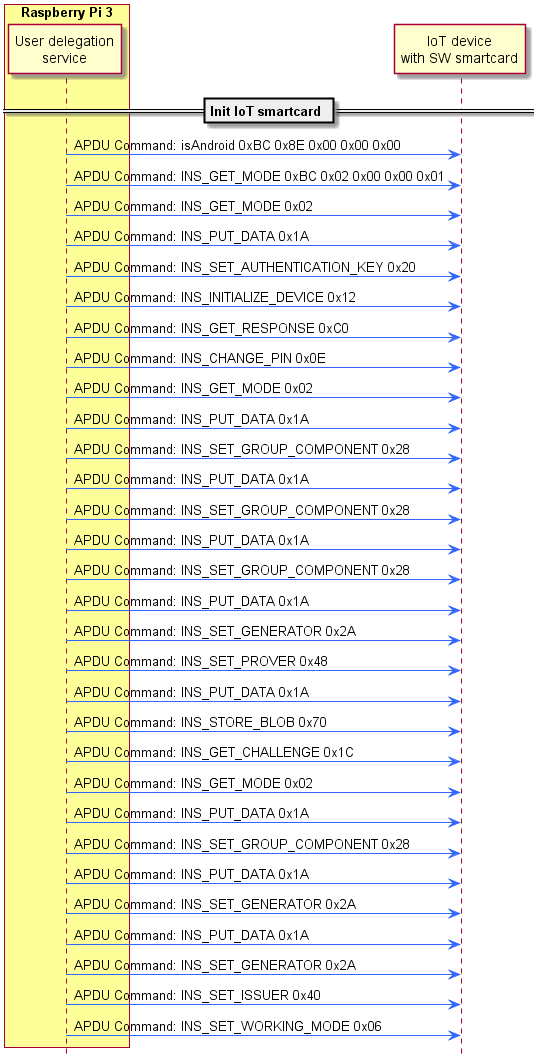
\includegraphics[width=0.9\linewidth]{gfx/UML/APDUsInitIoTSC}
	\end{center}
	\caption{Init IoT Smart Card APDU Commands exchanged.}
	\label{fig:APDUsInitIoTSC}
\end{figure}

\begin{figure}[bth]
	\begin{center}
		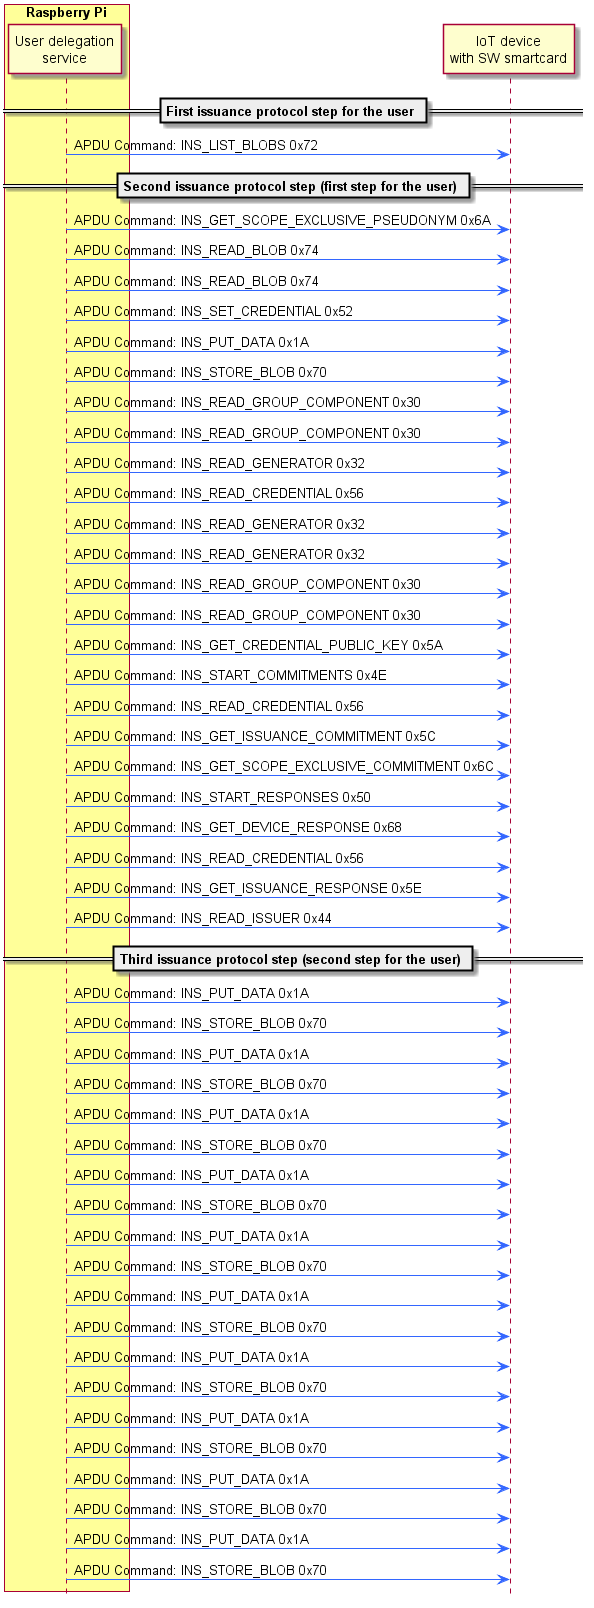
\includegraphics[width=0.78\linewidth]{gfx/UML/IssuanceAPDUs}
	\end{center}
	\caption{Issuance APDU Commands.}
	\label{fig:IssuanceAPDUs}
\end{figure}

\begin{figure}[bth]
	\begin{center}
		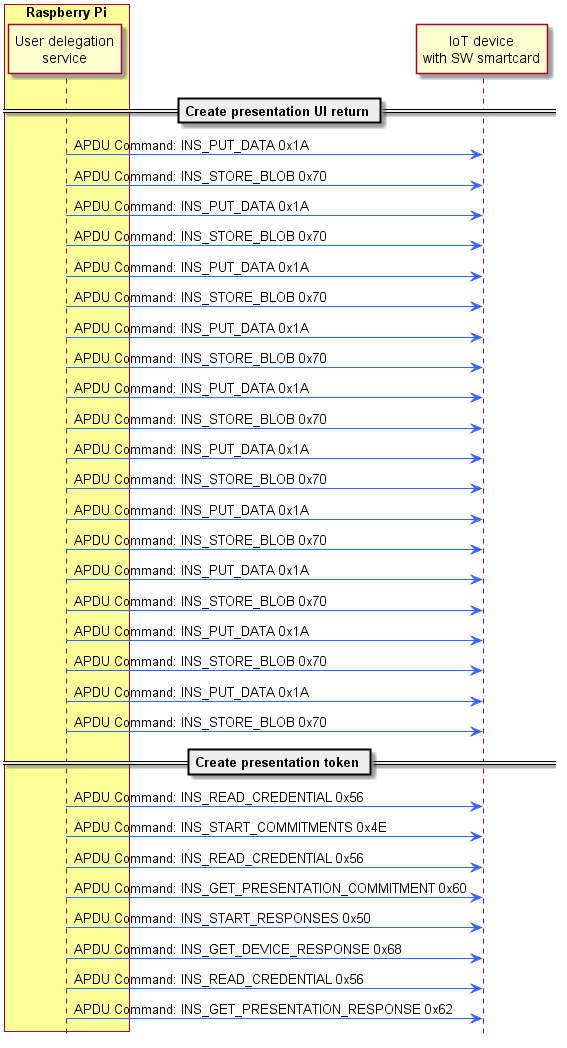
\includegraphics[width=\linewidth]{gfx/UML/APDUsProving}
	\end{center}
	\caption{Proving APDU Commands.}
	\label{fig:APDUsProving}
\end{figure}

\chapter{Guide on how to continue the project development}